\documentclass{article}
\usepackage{amsmath, graphicx}

\begin{document}
\title{Least Squares}
\author{}
\date{}
\maketitle

\section{Introduction}

Least squares is the workhorse of solving many data fitting problems such as regression.  The basic idea is to minimize the sum of squares error, which is often reasonable for some applications such as data corrupted by Gaussian noise, but often it is because squared error leads to efficient computational solutions.

The abstract optimization problem for linear least squares is as follows:
\begin{equation}
\min_x \quad \lVert{Ax - b}\rVert^2,
\end{equation}
where the matrix $A$ is $m \times n$, and the vector $b$ is $n \times 1$, and $m > n$.  So $A$ and $b$ are the knowns and $x$ is the unknown to be computed.  The matrix $A$ usually comes from the model of the problem, while $b$ are the measurements.  The problem is linear in $x$ because matrix multiplication is linear, hence the name linear least squares.

\section{Example}

Let's look at a simple example of fitting a quadratic function to noisy measurements as shown in Figure~\ref{fig:example}.  The actual model is a quadratic and the measurements are corrupted by Gaussian noise:
\begin{equation}
b_i = x_1 u_i^2 + x_2 u_i + x_3 + \epsilon_i,
\end{equation}
where $\epsilon_i$ is the noise.  Note that the input to the quadratic function is three-dimensional, $u^2$, $u$, and $1$, so that the formulation is linear in $x$.  In this example we have ten points, so $b$ is $10 \times 1$, $x$ is $3 \times 1$, so $A$ is $10 \times 3$.  The least squares estimate of $x$ is $(0.190787, 1.199769, -0.079463)^T$ and the true quadratic is $(0.183598, 1.226977, -0.089301)^T$, and Figure~\ref{fig:example} shows that with ten points for a three-dimensional problem, the least squares fit is pretty good (also in this example the noise was Gaussian which statiscally matches the squared error loss for least squares).

\begin{figure}
\centering
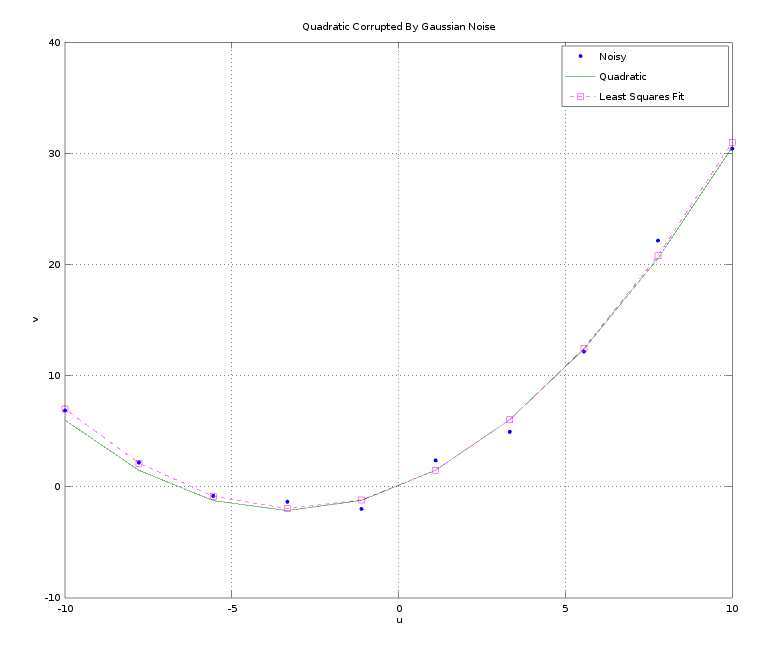
\includegraphics[width=4in]{example.png}
\caption{A quadratic function with measured points corrupted by noise.  The true quadratic is the green curve, while the noisy measurements are the blue dots.  The least squares estimate is show in magenta.}
\label{fig:example}
\end{figure}

\section{Computation}

To find the solution to the linear least squares problem, we can start with algebra.  From the theory we know that the cost function is quadratic because,
\begin{align}
\lVert{Ax - b}\rVert^2 &= (Ax - b)^T (Ax - b) \\
&= 2 x^T A^T A x -2 x^T A^T b + b^T b,
\end{align}
which means that there is a global minimum.
From calculus, we can take the derivative with respect to $x$, set it to zero, and algebraically determine $x$:
\begin{align}
E(x) &= 2 x^T A^T A x -2 x^T A^T b + b^T b \\
\frac{\partial E}{\partial x} &= 2 (A^T A x - A^T b) = 0 \\
A^T A x &= A^T b \\
x &= (A^T A)^{-1} A^T b.
\end{align}
Note that $A^T A$ is a square matrix of size $n \times n$.  The above equation is called the normal equation and is a fast way to compute the least squares solution; however it is not numerically the best because the $A^T A$ means that numbers get squared which can result in a loss of precision.  The above algebra also shows us that the solution $x$ is a linear function of the measurements $b$ because $A$ is known (from the model) so $A^T A$ is a known, fixed matrix.

We could also use gradient descent to find the solution:
\begin{equation}
x_{t+1} = x_t - \eta A^T(Ax_t - b),
\end{equation}
where $\eta$ is the learning/adjustment rate, and $A^T (Ax - b)$ is the gradient.  This kind of iterative method is sometimes useful for large-scale or other least squares problems.

The most robust way to solve the problem is to use the SVD:
\begin{align}
A & = USV^T \\
\lVert{Ax - b}\rVert^2 &= \lVert{USV^Tx - b}\rVert^2 \\
&= \lVert{U^T(USV^Tx - b)}\rVert^2 \\
&= \lVert{SV^Tx - U^Tb)}\rVert^2,
\end{align}
where the third line above is justified by the fact that $U$ is an orthogonal matrix which means it rotates a vector so rotating the residual vector $(Ax - b)$ doesn't change it's norm.
If we let $y = SV^Tx$, then we have the problem $\lVert{Sy - U^T b}\rVert$.  Now the normal equation above gives $y = (S^T S)^{-1} S^T U^T b$.  Note that that top rows $S$ is a diagonal matrix, so these computations are easy after the SVD.  Then we can recover $x$ by $x = Vy = VV^Tx$.

One could also use the QR factorization in a similar way.

\section{Interpretation}

As alluded to above, we can interpret the vector in the norm as a residual vector,
\begin{equation}
r =  Ax - b,
\end{equation}
which is why we want to minimize the norm or length of these residuals or approximation errors.  Each element of $r_i$ of $r$ can be interpreted as the error of the approximation for the $i$'th example, i.e., $r_i = a_i^T x - b_i$.  Without noise, all of the $r_i$ would be zero.  This is the row interpretation where each row $i$ of $A$ along with $b_i$ provides a datum to determine $x$.  In the column interpretation, we want to find an $x$ so that the linear combination of the columns of $A$ give the best approximation to $b$:
\begin{align}
Ax - b &= \left(\sum_j a_j x_j\right) - b
\end{align}

\end{document}
